%%
%% TODO: faire apparaitre les problematiques de recherche
%%

\begin{frame}<1-3>
    \frametitle{Background
       \only<2>{(Research Topics: Fault-Tolerance)}
       \only<3>{(Research Topics: Task-Based Runtime Systems)}
       \only<4>{(Funding Projects)}
       \only<5>{(software development and dissemination)}}

    \pgfplotsset{
        /pgf/number format/year/.style={fixed, 1000 sep={}}
    }

    \resizebox{\textwidth}{!}{
    \begin{tikzpicture}
        \draw[->,line width=.2mm,ultra thick] (0,0) -- (25,0);
        \foreach \x in {0,...,24}{\draw[thick] (\x,0.2)--(\x,-0.2);}
        \foreach \x in {0,4,...,24}{\pgfmathsetmacro\result{\x + 2000}\node at (\x,-0.4) {\pgfmathprintnumber[year]{\result}};}
    
        \fill[rounded corners=10pt,fill=black,fill opacity=0.2] (0,0.3) rectangle (3,-0.3);
        \node[align=center,text width=3cm] at (1.5,1) {Moniteur Normalien (Paris XI)};

        \fill[rounded corners=10pt,fill=black,fill opacity=0.2] (3,0.3) rectangle (4,-0.3);
        \node[align=center,text width=2cm] at (3.5,1) {ATER (Paris XI)};

        \fill[rounded corners=10pt,fill=black,fill opacity=0.2] (4,0.3) rectangle (24,-0.3);
        \node[align=center,text width=8cm] at (14,1) {Ma\^\i{}tre de Conf\'erences (Paris XI)};

        \fill[rounded corners=10pt,fill=black,fill opacity=0.2] (8,-0.7) rectangle (10,-1.3);
        \node[align=center,text width=3cm] at (9,-1) {D\'et. INRIA};

        \fill[rounded corners=10pt,fill=black,fill opacity=0.2] (10,-0.7) rectangle (20,-1.3);
        \node[align=center,text width=6cm] at (15,-1) {D\'etachement UTK};

        \fill[rounded corners=10pt,fill=black,fill opacity=0.2] (20,-0.7) rectangle (24,-1.3);
        \node[align=center,text width=3cm] at (22,-1) {Disponibilit\'e};

        \fill[rounded corners=10pt,fill=black,fill opacity=0.2] (8,-1.5) rectangle (10,-2.1);
        \node[align=center,text width=3cm] at (9,-1.8) {Vis. Sch. (UTK)};

        \fill[rounded corners=10pt,fill=black,fill opacity=0.2] (10,-1.5) rectangle (17,-2.1);
        \node[align=center,text width=6cm] at (13.5,-1.8) {Research Scientist II (UTK)};

        \fill[rounded corners=10pt,fill=black,fill opacity=0.2] (17,-1.5) rectangle (20,-2.1);
        \node[align=center,text width=3cm] at (18.5,-1.8) {Res. Dir. (UTK)};
    
        \fill[rounded corners=10pt,fill=black,fill opacity=0.2] (20,-1.5) rectangle (24,-2.1);
        \node[align=center,text width=4cm] at (22,-1.8) {Res. Ass. Pr. (UTK)};

        \fill[rounded corners=10pt,fill=red,fill opacity=0.2] (0,-2.5) rectangle (6,-3.1);
        \node[align=center,text width=6cm] at (3,-2.8) {Self-Stabilization, Dist. Alg.};

        \fill[rounded corners=10pt,fill=red,fill opacity=0.2] (7,-2.5) rectangle (11,-3.1);
        \node[align=center,text width=6cm] at (9,-2.8) {``D\'efi S\'ecurit\'e''};

        \fill[rounded corners=10pt,fill=blue,fill opacity=0.2] (13,-2.5) rectangle (24,-3.1);
        \node[align=center,text width=12cm] at (18.5,-2.8) {Performance Modeling for Fault Tolerance};

    \only<4>{
        \fill[fill=red,fill opacity=.4] (7,-3.5) rectangle (11,-3.7);
        \node[align=center,text width=3cm] at (9,-3.6) {\textbf{PI} SAFE-OS (ANR)};

        \fill[fill=blue,fill opacity=.4] (16,-3.5) rectangle (20,-3.7);
        \node[align=center,text width=3cm] at (18,-3.6) {\textbf{PI} SMURFS (NSF)};
    }
    
        \fill[rounded corners=10pt,fill=blue,fill opacity=0.2] (3,-4.1) rectangle (10,-4.7);
        \node[align=center,text width=6cm] at (6.5,-4.4) {Rollback recovery in MPICH};

        \fill[rounded corners=10pt,fill=brown,fill opacity=0.2] (10,-4.1) rectangle (24,-4.7);
        \node[align=center,text width=18cm] at (17,-4.4) {Task-Based Runtime Systems};

    \only<5>{
        \fill[fill=blue,fill opacity=.6] (3,-5.3) rectangle (10,-5.5);
        \node[align=left,text width=6cm,color=blue,anchor=west] at (3,-5.1) {\textbf{MPICH-V}};
        \fill[fill=yellow,fill opacity=1] (8,-5.4) circle (3pt);
        \node[align=center,text width=6cm,color=blue] at (8,-5.1) {MPICH (distcont.)};

        \fill[fill=brown,fill opacity=.6] (10,-5.3) rectangle (13,-5.5);
        \node[align=left,text width=6cm,color=brown,anchor=west] at (10,-5.1) {\textbf{DAGuE}};
        \fill[fill=brown,fill opacity=.6] (13,-5.3) rectangle (24,-5.5);
        \node[align=left,text width=6cm,color=brown,anchor=west] at (13,-5.1) {\textbf{PaRSEC}};
        \node[align=left,anchor=south west,color=brown] at (25,-5.1) {$\left\{\begin{tabular}{l}\textrm{DPLASMA (UTK)}\\\textrm{Chameleon (INRIA)}\\\textrm{PaSTIX (INRIA)}\\\textrm{HiCMA (KAUST)}\\\textrm{MADNESS (SBU)}\\\textrm{NWChemEx (NWU)}\end{tabular}\right.$};
    }
    
    \only<4>{
        \fill[fill=blue,fill opacity=.4] (6,-5.1) rectangle (9,-5.3);
        \node[align=center,text width=3cm] at (7.5,-5.2) {\textbf{coPI} QosCosGrid (STREP)};
        \fill[fill=brown,fill opacity=.4] (16,-5.1) rectangle (23,-5.3);
        \node[align=center,text width=3cm] at (19.5,-5.2) {\textbf{coPI} ECP PaRSEC (DoE)};
    }

        \fill[rounded corners=10pt,fill=red,fill opacity=0.2] (2,-5.7) rectangle (7,-6.3);
        \node[align=center,text width=6cm] at (4.5,-6.0) {App. Prob. Model Checking};

        \fill[rounded corners=10pt,fill=blue,fill opacity=0.2] (8,-5.7) rectangle (24,-6.3);
        \node[align=center,text width=12cm] at (16,-6.0) {Fault Tolerant MPI, Application-Specific FT for HPC};

    \only<5>{
        \fill[fill=blue,fill opacity=.6] (11,-6.9) rectangle (24,-7.1);
        \node[align=left,text width=6cm,color=blue,anchor=west] at (11,-6.7) {\textbf{User-Level Failure Mitigation}};
        \fill[fill=yellow,fill opacity=1] (21,-7.0) circle (3pt);
        \node[align=right,anchor=east,text width=6cm,color=blue] at (21.5,-6.7) {Open MPI};
        \fill[fill=yellow,fill opacity=1] (22,-7.0) circle (3pt);
        \node[align=left,anchor=west,text width=6cm,color=blue] at (21.5,-6.75) {MPICH};
        \node[align=left,anchor=west,color=blue] at (25,-6.7) {$\left\{\begin{tabular}{l}\textrm{Fenix (SNL)}\\\textrm{CRAFT (RRZE)}\\\textrm{Resilient X10 (ANU)}\\\textrm{Hadoop - FT-MRMPI (U.Col)}\\\textrm{SAP database (Germany)}\\\textrm{NR-MPI (NUDT, China)}\end{tabular}\right.$};
    }

    \only<4>{
        \fill[fill=blue,fill opacity=.4] (17,-6.7) rectangle (23,-6.9);
        \node[align=center,text width=3cm] at (19,-6.8) {\textbf{coPI} EVOLVE (NSF)};
    }
        

        \fill[rounded corners=10pt,fill=brown,fill opacity=0.2] (12,-7.3) rectangle (24,-7.9);
        \node[align=center,text width=18cm] at (18,-7.6) {Programming Interface for Irregular Task Systems};

    \only<1,2>{
        \node[align=left,anchor=south west,color=white,opacity=0] at (25,-8.3) {$\left\{\begin{tabular}{l}\textrm{Hadoop - FT-MRMPI (U.Col)}\\\textrm{Hadoop - FT-MRMPI (U.Col)}\\\textrm{Hadoop - FT-MRMPI (U.Col)}\end{tabular}\right.$};
    }
    \only<5>{
        \fill[fill=brown,fill opacity=.6] (13,-8.5) rectangle (24,-8.7);
        \node[align=left,text width=6cm,color=brown,anchor=west] at (13,-8.3) {\textbf{Template Task Graph}};
        \node[align=left,anchor=north west,color=brown] at (25,-8.3) {$\left\{\begin{tabular}{l}\textrm{TiledArray (VT)}\\\textrm{MADNESS (SBU)}\\MPQC (VT)\end{tabular}\right.$};
    }
    \only<4>{
        \fill[fill=brown,fill opacity=.4] (14,-8.3) rectangle (19,-8.5);
        \node[align=center,text width=3cm] at (16.5,-8.4) {\textbf{coPI} TESSE (NSF)};
        \fill[fill=brown,fill opacity=.4] (19,-8.3) rectangle (25,-8.5);
        \node[align=center,text width=3cm] at (22,-8.4) {\textbf{coPI};\textbf{PI} EPEXA (NSF)};
    }
    
        \fill[rounded corners=10pt,fill=brown,fill opacity=0.2] (15,-8.9) rectangle (24,-9.5);
        \node[align=center,text width=18cm] at (19.5,-9.2) {Memory-Constrained Scheduling of Tasks};

    \end{tikzpicture}}

    \begin{overlayarea}{\linewidth}{0cm}
    \only<2>{%
      \vspace{-6cm}
      \begin{center}
        \begin{minipage}{.9\linewidth}
          \begin{block}{Research Topics: Fault Tolerance}
            Two complementary approaches to Fault Tolerance
              \begin{itemize}
              \item General Purpose Fault Tolerance
                \begin{itemize}
                \item Checkpointing and rollback-recovery
                  \begin{itemize}
                  \item Experimental approach: implementing new protocols and evaluating them in 'real' applications / deployments
                  \item Performance models approach: designing mathematical models to project performance at scale or under new assumptions
                  \end{itemize}
                \end{itemize}
              \item Application-Specific Fault Tolerance
                \begin{itemize}
                \item Design / adapt communication middlewares to write fault-tolerant applications
                \item Design and evaluate new fault-tolerance schemes for parallel applications
                \end{itemize}
              \end{itemize}
          \end{block}
        \end{minipage}
      \end{center}
    }
    \only<3>{%
      \vspace{-6cm}
      \begin{center}
        \begin{minipage}{.9\linewidth}
          \begin{block}{Research Topics: Task Based Runtime Systems}
            \begin{itemize}
            \item Main topic: portable programmability for HPC
                \begin{itemize}
                \item Networks with deep hierarchies / Manycore / NUMA / Accelerators
                \item Separation of concerns: going beyond MPI+X
                \item Management of asynchrony
                \item Overlap of computations and data movement
                \end{itemize}
            \item Related topics:
                \begin{itemize}
                \item Expression of parallelism / Programming Interfaces
                \item Out-of-(accelerator) core memory programming / Memory-Constrained algorithms
                \item Multiresolution computation with dynamic decision
                \item Sparse and computation-dependent task systems
                \end{itemize}
            \end{itemize}
          \end{block}
        \end{minipage}
      \end{center}
    }
  \end{overlayarea}

\end{frame} 
    
%% \frame{
%%   \frametitle{Overview: General Purpose Fault Tolerance}

%%   \begin{columns}
%%     \begin{column}{.5\textwidth}
%%       Experimental approach: MPICH-V
%%       \begin{itemize}
%%       \item Coordinated Rollback-Recovery
%%         \begin{itemize}
%%         \item Blocking/Non Blocking
%%         \end{itemize}
%%       \item Uncoordinated Rollback-Recovery
%%         \begin{itemize}
%%         \item Message Logging
%%         \item Optimistic / Pessimistic / Causal
%%         \end{itemize}
%%       \item Hierarchical Approach
%%       \end{itemize}
%%     \end{column}
%%     \begin{column}{.5\textwidth}
%%       Performance Models for Rollback-Recovery
%%       \begin{itemize}
%%       \item \textcolor{blue}{Young-Daly}
%%       \item \textcolor{blue}{Hierarchical Checkpointing}
%%       \item In-Memory Checkpointing
%%       \item Managing I/O Contention
%%       \end{itemize}
%%     \end{column}
%%   \end{columns}
%% }

%% \frame{
%%   \frametitle{Overview: Application-Specific Fault-Tolerance}
  
%%   \begin{columns}
%%     \begin{column}{.5\textwidth}
%%       User-Level Failure Mitigation
%%       \begin{itemize}
%%       \item Specification / Standardization
%%       \item \textcolor{blue}{Failure Detection}
%%       \item \textcolor{blue}{Consensus}
%%       \item Silent Errors
%%       \end{itemize}
%%     \end{column}
%%     \begin{column}{.5\textwidth}
%%       Roll-forward fault-tolerance
%%       \begin{itemize}
%%       \item ABFT for dense matrix factorization
%%       \item Composite Approach: ABFT \& Checkpointing
%%       \item Moldable Applications
%%       \end{itemize}
%%     \end{column}
%%   \end{columns}
%% }
    
%% \frame{
%%   \frametitle{Background (Task-Based Runtime Systems)}
  
%%   \begin{columns}
%%     \begin{column}{.5\textwidth}
%%       Parallel Runtime Scheduler and Execution Controller (PaRSEC)
%%       \begin{itemize}
%%       \item Micro task (task scheduling overhead $\sim 200ns$)
%%       \item Distributed (runs with thousands of nodes)
%%       \item Hybrid (Intel, AMD, NVIDIA GPUs)
%%       \item Implicit data movement (from device to device, in the background)
%%       \item Multiple programming interfaces
%%         \begin{itemize}
%%         \item Parameterized Task Graphs
%%         \item Dynamic Task Discovery
%%         \item Template Task Graphs
%%         \end{itemize}
%%       \end{itemize}
%%     \end{column}
%%     \begin{column}{.5\textwidth}
%%       \begin{itemize}
%%       \item Applications:
%%         \begin{itemize}
%%         \item Dense Linear Algebra (DPLASMA)
%%         \item Sparse Linear Algebra (PaStiX, TiledArray)
%%         \item Quantum Chemistry (NWChem, MPQC)
%%         \item Multi-representation (HiCMA)
%%         \end{itemize}
%%       \item Node-to-node migratable tasks
%%       \item Resilient extensions
%%         \begin{itemize}
%%         \item Resilient to Silent Data Corruptions via Algorithm-Based Fault-Tolerance validation
%%         \item Task-based checkpoint and partial rollback-recovery
%%         \end{itemize}
%%       \end{itemize}
%%     \end{column}
%%   \end{columns}
%% }

